\section{Ziel}
\label{sec:ziel}

Im folgenden Experiment soll mit Hilfe der Emissionsspektren der Alkalimetalle Natrium, Kalium und Rubidium die Abschirmungszahl $\sigma$ bestimmt werden.

\section{Theorie}
\label{sec:theorie}

\subsection{Emissionsspektren}
\subsubsection{Ein-Elektron-Spektren}
Für Alkalimetalle gilt die Ein-Elektron-Näherung, da über abgeschlossenen Elektronenschalen jeweils nur ein äußeres Elektron existiert, welches als Leuchtelektron bezeichnet wird. Es wird angenommen, dass die inneren Elektronen die Ladung der Protonen im Atomkern abschirmen. Es gilt:
\begin{equation}
  z_\mathrm{eff} = z-\sigma.
\end{equation}
Dabei ist $z$ die Kernladungszahl des jeweiligen Atoms.

\subsubsection{Strahlungsenergien}
Um die Energieniveaus hinreichend genau beschreiben zu können, wird angenommen, dass diese von der Hauptquantenzahl $n$ und den Nebenquantenzahlen $l$ und $j$ abhängig sind. $l$ wird als Bahndrehimpulsquantenzahl und $j$ als zum Spin des Elektrons zugehörige Quantenzahl bezeichnet. Der Spin eines Elektrons wird auch Eigendrehimpuls genannt, da er auch vorliegt, wenn das Elektron keine kinetische Energie besitzt. Er kann nur den Wert $s=\pm\frac{1}{2}$ annehmen.
Dass es sich bei den Emissionsspektren um Linienspektren handelt, kann wie folgt erklärt werden:
Das äußere Elektron kann durch Zuführen von Energie auf ein höheres Energieniveau gelangen. Gelangt es zurück auf das niedrigere Energienniveau, wird die Energiedifferenz als Elektromagnetische Strahlung emittiert. Da nur bestimmte Energieniveaus existieren, ergibt sich ein Linienspektrum.
Mit Hilfe der Schrödinger-Gleichung
\begin{equation}
  \left(\sum_{i}\frac{P_\mathrm{i}^2}{2m_\mathrm{i}}+U\right)\psi =  E\psi
\end{equation}
mit $\psi$ als Wellenfunktion, $P_\mathrm{i}$ als Impulsoperator, $U$ als potentielle Energie und $m_\mathrm{i}$ als Masse, wird eine Gleichung für die Energiewerte in Abhängigkeit der Quantenzahlen hergeleitet. Für den Hamilton-Operator des Atoms gilt:
\begin{equation}
  H=\sum_{i}\frac{P_\mathrm{i}^2}{2m-\mathrm{i}} + U.
\end{equation}
Bei Atomen mit großer Kernladungszahl müssen realtivistische Effekte berücksichtigt werden. Zur Vereinfachung werden diese als Störung behandelt. Schließlich ergibt sich für die Enegieeigenwerte
\begin{equation}
  E_\mathrm{n,l,j} = -R_\infty \left(\frac{(z-\sigma)^2}{n^2}+\alpha^2\frac{(z-\sigma)^4}{n3}\left(\frac{2}{2l+1}-\frac{3}{4n}-\frac{j(j+1)-l(l+1)-(3/4)}{l(l+1)(2l+1)}\right)\right).
\end{equation}
$R_\infty$ ist die Rydbergenergie und $\alpha$ die Sommerfeldsche Feinstrukturkonstante. Unter Berücksichtigung der Tatsache, dass $j=l \pm \frac{1}{2}$, folgt:
\begin{equation}
  \label{eqn:sommerfeld1}
  E_\mathrm{n,j}= -R_\infty \left(\frac{(z-\sigma)^2}{n^2}+\alpha^2\frac{(z-\sigma)^2}{n^3}\left(\frac{1}{j+(1/2)} -\frac{3}{4n}\right)\right).
\end{equation}
Für $l=0$ gilt:
\begin{equation}
  \label{eqn:sommerfeld2}
  E_\mathrm{n,(1/2)} = -R_\infty \left(\frac{(z-\sigma)^2}{n^2}+\alpha^2\frac{(z-\sigma)^4}{n^3} \left( 1-\frac{3}{4n}\right)\right).
\end{equation}
Die Gleichungen \ref{eqn:sommerfeld1} und \ref{eqn:sommerfeld2} werden Sommerfeldsche Feinstrukturformeln in erster Näherung genannt.

\subsubsection{Auswahlregeln}
Für die Übergänge zwischen den Energieniveaus gelten unterschiedliche Übergangswahrscheinlichkeiten. Es existieren keine Übergänge ohne Änderung des Bahndrehimpulses $l$. Außerdem muss immer $\Delta l = \pm 1$ gelten. Übergänge ohne Änderung der Spinquantenzahl $j$ sind möglich, allerdings unwahrscheinlich. Die Änderung der Hauptquantenzahl $n$  ist uneingeschränkt. Jedoch werden Übergänge mit großem $\Delta n$ zunehmend unwahrscheinlicher.
Die in Alkalispektren auftretenden Dublett-Strukturen, die sich durch zwei nah nebeneinander liegende Linien äußern könnnen darauf zurückgeführt werden, dass Energieniveaus mit gleichem $l$ udn unterschiedlichem $j$ in einem kleineren Abstand zueinander liegen als die mit unterschiedlichem $l$.

\begin{figure}
  \centering
  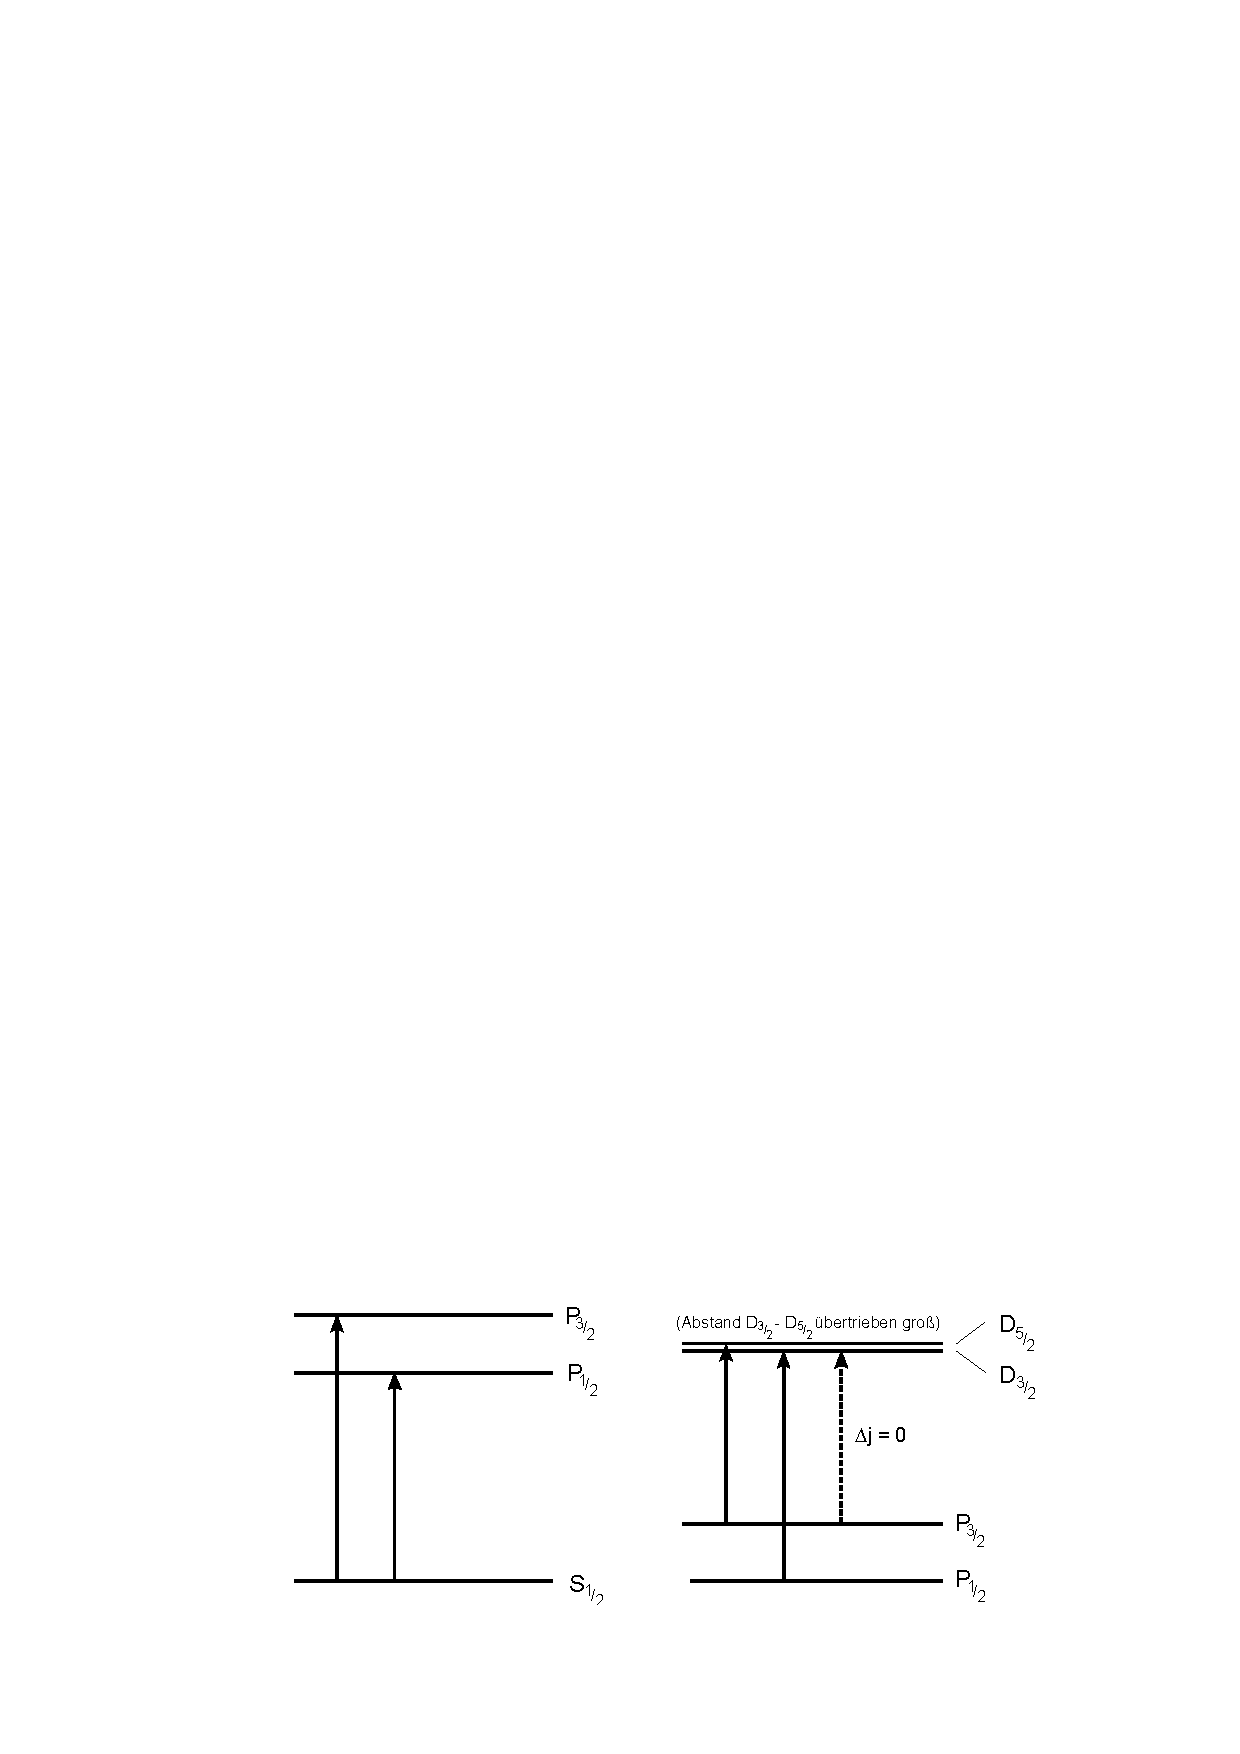
\includegraphics[scale=0.8]{content/übergänge.pdf}
\caption{Mögliche Übergänge in Ein-Elektron-Spektren\cite{anleitung605}.}
  \label{fig:übergänge}
\end{figure}
Abbildung \ref{fig:übergänge} zeigt mögliche Übergänge zwischen den Energieniveaus.

\subsubsection{Abschirmungszahlen}
Bei der Abschirmungszahl soll zwischen der Konstante der vollständigen Abschirmung $\sigma_1$, welche alle Elektronen berücksichtigt und er Konstante der inneren Abschirmung $\sigma_2$, welche nur die Elektronen auf der Schale des Leuchtelektrons berücksichtigt, unterschieden werden. Um $\sigma_2$ bestimmen zu können, muss der Abstand $\Delta E_\mathrm{D}$ der beiden Linien des Dubletts bekannt sein.
\begin{equation}
  \label{eq:ED1}
  \Delta E_\mathrm{D} = \frac{R_\infty \alpha^2}{n^3}(z-\sigma_2)^4 \frac{1}{l(l+1)}
\end{equation}

Mit $E=\frac{hc}{\lambda}$ ($h$ ist das Planksche Wirkungsquantum, $c$ die Lichtgeschwindigkeit im Vakuum, $\lambda$ die Wellenlänge) folgt für $\Delta E_\mathrm{D}$:
\begin{equation}
  \label{eq:ED2}
\Delta E_\mathrm{D} = hc \left( \frac{1}{\lambda}-\frac{1}{\lambda'}\right) \approx hc \frac{\Delta \lambda}{\lambda^2}
\end{equation}

\subsection{Gitter}
Ein Gitter setzt sich aus einer Vielzahl von Spalten in einem lichtundurchlässigem Material zusammen. Trifft Licht auf das Gitter, wird es gebeugt (siehe Abbildung \ref{fig:gitter}). Der Winkel, um den das Licht abgelenkt wird, ist abhängig von der Gitterkonstante $g$ und der Wellenlänge $\lambda$ des einfallenden Lichts. Es entstehen Maxima und Minima unterschiedlicher Ordnungen $k$.
Es gibt Haupt- und Nebenmaxima. Durch Erhöhung der Anzahl der Gitteröffnungen kann der Abstand zwischen zwei Minima verringert werden. Somit können die Nebenmaxima bei einer großen Anzahl von Öffnungen vernachlässigt werden. Zwischen dem Winkel, unter welchem ein Hauptaximum entsteht, und der Wellenlänge besteht folgender Zusammenhang:
\begin{equation}
  \sin \phi = k\frac{\lambda}{g}.
\end{equation}

\begin{figure}
  \centering
  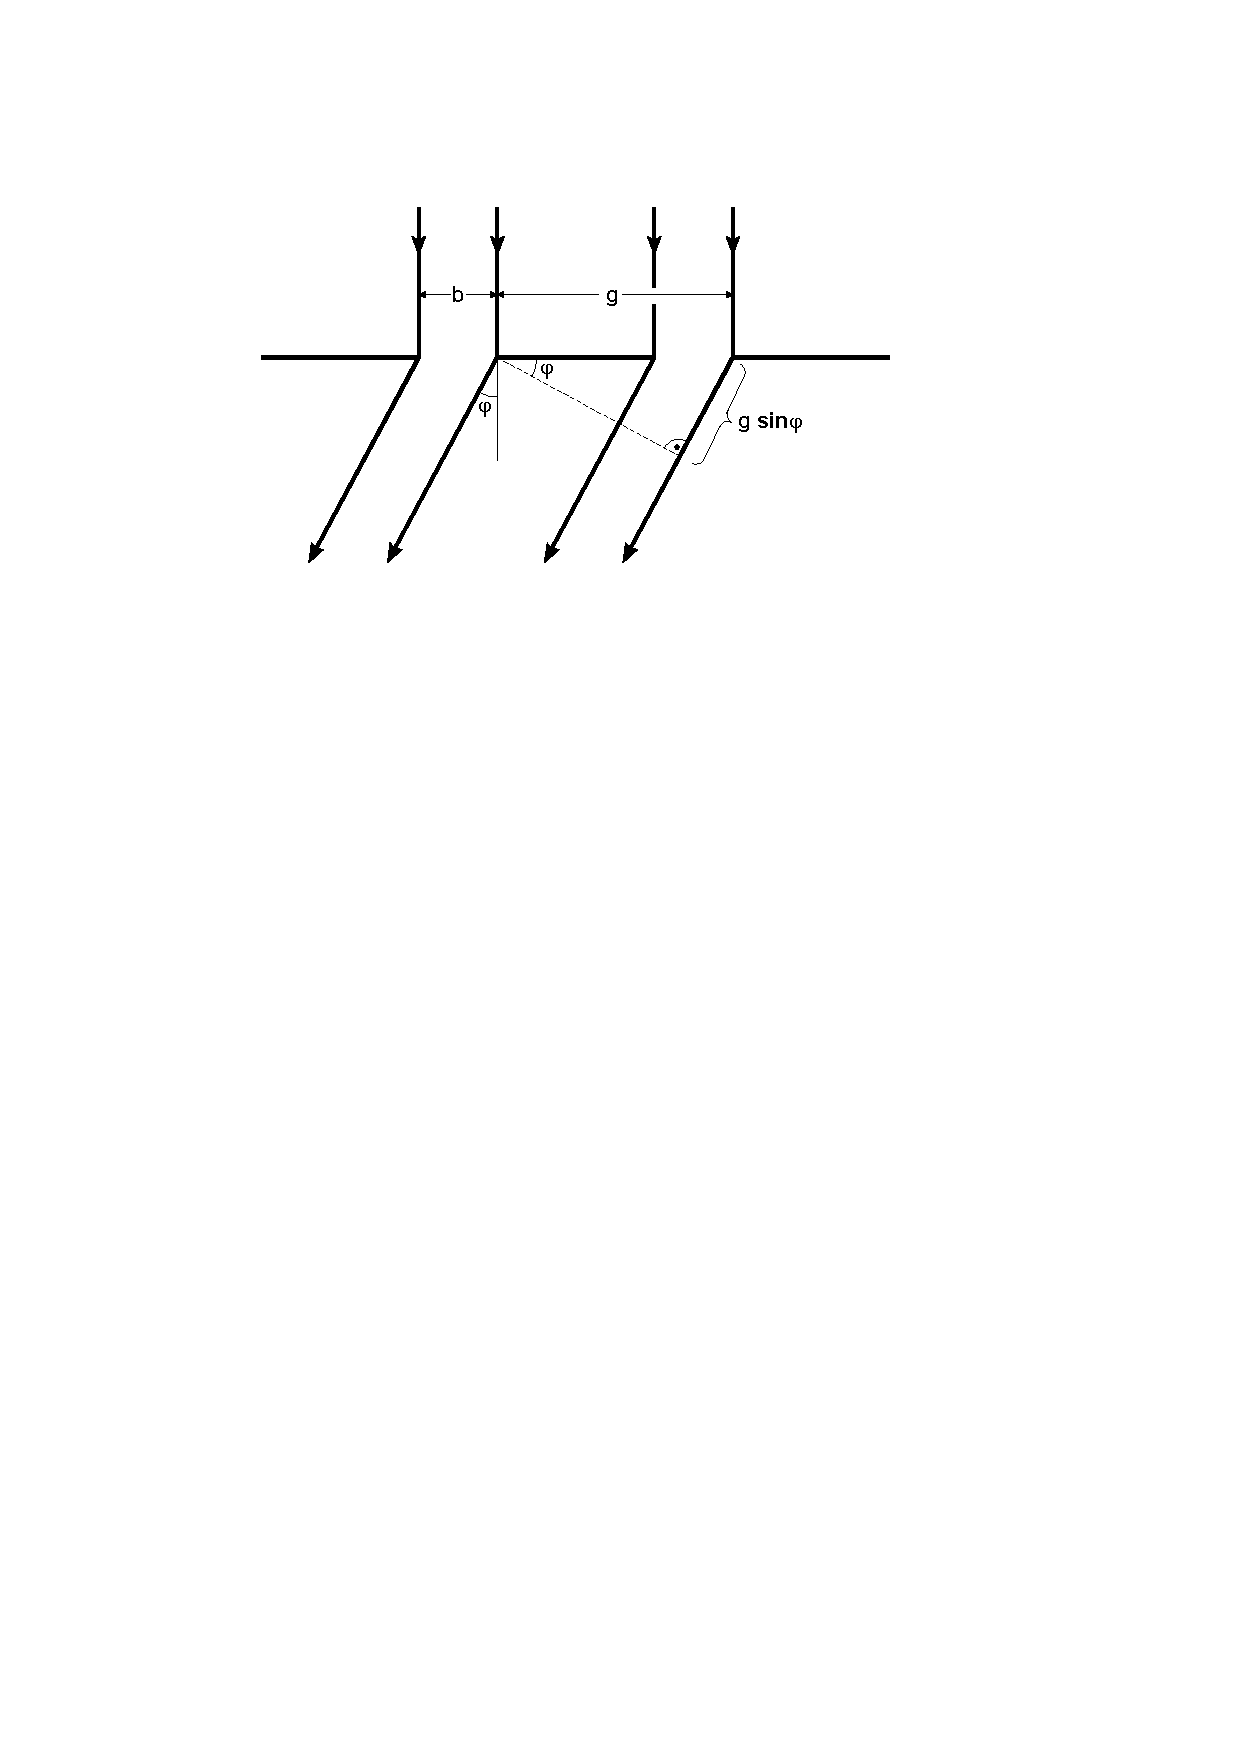
\includegraphics[scale=0.8]{content/gitter.pdf}
\caption{Beugung einer ebenen Welle an Spaltöffnungen der Breite $b$\cite{anleitung605}.}
  \label{fig:gitter}
\end{figure}
